\documentclass{article}
\usepackage[T2A]{fontenc}
\usepackage[utf8]{inputenc}
\usepackage[english, russian]{babel}
\usepackage{diplstyle}
\usepackage{geometry}
\usepackage{floatflt}
\usepackage[usenames,dvipsnames]{color}
\usepackage[numbered]{mcode}
\usepackage{subfigure}
\usepackage{listings, xcolor}
\usepackage[]{algorithm2e}
\usepackage{hyperref}
\usepackage{indentfirst}
\usepackage{enumitem}
\usepackage{dirtree}
\usepackage{minted}
% \hypersetup{
%     colorlinks,
%     citecolor=black,
%     filecolor=black,
%     linkcolor=black,
%     urlcolor=black
% }s	
% \usepackage{mathptmx}

\geometry{left=3cm}
\geometry{right=1.5cm}
\geometry{top=2cm}
\geometry{bottom=2cm}
\pagestyle{plain}
\parindent=1.25cm
\linespread{1.3}

\begin{document}
%\thispagestyle{empty}
\vskip 15 mm
\centerline{\footnotesize{\bf{Министерство науки высшего образования Российской Федерации}}}
\centerline{\footnotesize{{ФЕДЕРАЛЬНОЕ ГОСУДАРСТВЕННОЕ АВТОНОМНОЕ ОБРАЗОВАТЕЛЬНОЕ УЧРЕЖДЕНИЕ}}}
\centerline{\small{{ВЫСШЕГО ОБРАЗОВАНИЯ}}}
\centerline{{\bf{«НАЦИОНАЛЬНЫЙ ИССЛЕДОВАТЕЛЬСКИЙ УНИВЕРСИТЕТ ИТМО»}}}
\centerline{{\bf{(Университет ИТМО)}}}
\centerline{Факультет информационных технологий и программирования}

\vskip 30 mm
\centerline{\LARGE{ОТЧЕТ}}
\centerline{\LARGE{О НАУЧНО-ИССЛЕДОВАТЕЛЬСКОЙ РАБОТЕ}}
\vskip 2 mm
\centerline{\large{по теме:}}
\vskip 2 mm
\centerline{\large\bf{ПРОЕКТИРОВАНИЕ И РЕАЛИЗАЦИЯ РАСЧЕТНОГО МОДУЛЯ}}
\vskip 1 mm
\centerline{\large\bf{ДЛЯ СИСТЕМЫ АВТОМАТИЧЕСКОГО ФОРМИРОВАНИЯ}}
\vskip 1 mm
\centerline{\large\bf{ГЕНЕРАЛЬНЫХ ПЛАНОВ}}
\vskip 1 mm
\centerline{\large\bf{ПЛОЩАДНЫХ ОБЪЕКТОВ КАПИТАЛЬНОГО СТРОИТЕЛЬСТВА}}
\vskip 35 mm
\centerline{\large{СПИСОК ИСПОЛНИТЕЛЕЙ}}
\vskip 2 mm
\large{
\noindent
Научный руководитель, \\
Университет ИТМО, \\
факультет информационных технологий и программирования, \\
преподаватель \hskip 112 mm Пантенков С.~А.\\
\vskip 2 mm \noindent
Студент, \\
Направление подготовки 09.04.02 \\
Информационные системы и технологии, \\
Академическая группа M42051 \hskip 80 mm Степанов С.~В.\\
\vfill \hfil \break
\centerline{\large Санкт-Петербург } \centerline{ 2022 }}
\newpage

%\subsection*{\Large{Реферат}}
Данный отчет состоит из 16 страниц.
Содержит в себе 3 иллюстрации, 4 листинга кода, 7 использованных источников.
В данном отчете описывается проектирование и реализация сервиса, обеспечивающего
преобразование данных предметной области в объекты математической библиотеки \textbf{nd\_plan},
и имеющий возможность запускать методы данной библиотеки, учитывая особенности их выполнения.
В рамках данной работы были проанализированы функциональные и нефункциональные требования, спроектирована
архитектура сервиса и реализована запроектированная архитектура.
%\newpage
%\large{\tableofcontents}
%\newpage
%\section*{\large{ОПРЕДЕЛЕНИЯ, ОБОЗНАЧЕНИЯ И СОКРАЩЕНИЯ}}
\addcontentsline{toc}{section}{\large{ОПРЕДЕЛЕНИЯ, ОБОЗНАЧЕНИЯ И СОКРАЩЕНИЯ}}

В данной работе применяют следующие термины с соответствующими определениями.

\textit{Генеральный план (генплан, ГП)} в общем смысле —
проектный документ, на основании которого осуществляется планировка,
застройка, реконструкция и иные виды градостроительного освоения территорий.
Основной частью генерального плана (также называемой собственно генеральным планом)
является масштабное изображение, полученное методом графического наложения чертежа
проектируемого объекта на топографический,
инженерно-топографический или фотографический план территории\cite{CapitalBuilding}.


\textit{Площадными объектами капитального строительства (ПО)} в данной работе называются
здания, строения, сооружения, а также объекты, строительство которых не завершено, за исключением некапитальных строений,
сооружений и неотделимых улучшений земельного участка (замощение, покрытие и другие)\cite{CapitalBuilding}.


\textit{Здание} — результат строительства, представляющий собой объемную строительную систему,
имеющую надземную и (или) подземную части, включающую в себя помещения,
сети инженерно-технического обеспечения и системы инженерно-технического обеспечения и предназначенную для проживания и
(или) деятельности людей, размещения производства, хранения продукции или содержания животных\cite{SafetyBuildings}.


\textit{Сооружение} — результат строительства,
представляющий собой объемную, плоскостную или линейную строительную систему,
имеющую наземную, надземную и (или) подземную части, состоящую из несущих,
а в отдельных случаях и ограждающих строительных конструкций и предназначенную для выполнения
производственных процессов различного вида, хранения продукции, временного пребывания людей,
перемещения людей и грузов\cite{SafetyBuildings}.


\textit{Строения} — общее понятие зданий и сооружений\cite{CivilCode}.

%\newpage
%\section*{\Large{Введение}}
\addcontentsline{toc}{section}{Введение}
Автоматическое формирование генерального плана площадного объекта капитального строительства является чрезвычайно
сложной задачей, как в алгоритмическом, так и в технологическом плане.
Генеральный план помимо расстановки сооружений содержит расположение различных трубопроводов, линий электропередач,
внутриплощадочных проездов, пожарных гидранты и прочих объектов, необходимых для функционирования того или иного
промышленного объекта.

Для того, чтобы задача была выполнена качественно, требуется применение математического аппарата. Математический
аппарат подразумевает приведение объектов, которыми оперирует бизнес, к абстракциям,
которые могут использованы в алгоритмах. Именно эти алгоритмы, которые несколько отдалены от понятий бизнеса и являются
основным ядром и функционалом системы. Все эти алгоритмы выделены в отдельную математическую библиотеку.

Как и любая математически сложная задача, она обладает следующими свойствами:
\begin{itemize}
    \item долгое время выполнения;
    \item высокая загруженность центрального процессора;
    \item высокое потребление оперативной памяти.
\end{itemize}

Требуется создать прослойку, которая сможет превращать объекты технологической модели данных в объекты математической
библиотеки, а также сможет запускать математические методы, учитывая их особенности выполнения.

%\section*{\Large{Постановка задачи}}
\addcontentsline{toc}{section}{\Large{Постановка задачи}}

% Так как генплан дофига сложный то нужна типа система, которая сможет помочь проектировщикам в их нелегком деле
% Но чтобы создать эту систему нужно дофига усилий

Процесс проектирования генерального плана площадного объекта является непростым
и требует большого объема знаний от специалиста, как в сфере государственного законодательства,
так и сфере правил эксплуатации сооружений.
Из-за большого количества объектов, используемых на генплане, специалисту легко допустить ошибку,
которая может быть замечена лишь на поздних этапах проекта.

Набор правил минимальных допустимых расстояний между объектами является одним из основных критериев,
которым руководствуются инженеры-проектировщики при размещении объекта на генплане.
Основное требование заключается в нахождении объекта на достаточном удалении от остальных,
с целью снижения риска для здоровья и жизни людей во время эксплуатации площадного объекта.
Примером подобных правил являются
требования к ограничению распространения пожара. \cite{Fire}
Они вычисляются на основе класса конструктивной пожарной опасности и степени огнестойкости.
Но для предотвращения распространения пожара также важны
активные средства, какими являются пожарные гидранты, количество и производительность которых определяется
дополнительно строительным объемом сооружений.

Также при проектировании важно учитывать различные технические ограничения используемых объектов.
Например, для трубопроводов таковыми являются диаметр, радиус поворота и пр.

У каждого проектного решения есть стоимость, включающая в себя как капитальные затраты, так и эксплуатационные.
CAD-системы не обладают встроенным инструментом стоимостного моделирования,
поэтому инженер не может заранее узнать,
насколько его решение экономически эффективно для площадного объекта в целом,
так как полноценный расчёт затрат происходит позже на этапе формирования сметы
и оказывается несколько отделенным от процесса проектирования.

Таким образом, рынок нуждается в системе способной как формировать генеральные планы в автоматическом режиме,
так и верифицировать существующие решения в соответствии с заданным набором правил,
а также способной оценивать и сравнивать решения с точки зрения экономической эффективности.

Создание инструмента для аналитики и формирования генпланов площадных объектов позволит снизить
капитальные затраты при строительстве промышленных объектов благодаря повышению качества проектирования.
Подобный инструмент позволит сравнить несколько различных вариантов планировок промышленного объекта,
чтобы выбрать оптимальный по ряду критериев, а также получить обоснование,
почему выбранный вариант планировки действительно является оптимальным.

Формирование генплана площадного объекта в автоматическом режиме
на основе заданного перечня сооружений, технологических связей,
формы и размера участка местности, доступного для застройки,
а также требований нормативной документации является
крайне сложной алгоритмической задачей, для которой отсутствуют готовые методики решения.

Процесс создания системы для решения подобной задачи требует
проведения массы исследований в сфере алгоритмов и может занимать не один год.
В силу столь длительных сроков проведения научных изысканий остро стоит вопрос по созданию инструмента,
способного упростить данный процесс.
Процесс исследований напрямую связан с взаимодействием с техническими экспертами
в области проектирования генеральных планов.
Для достижения высоких результатов в сфере исследований очень важно получение обратной связи,
качество и оперативность которой позволяет сделать процесс исследований максимально продуктивным.

\textit{Целью} данной работы является
упрощение процесса проведения научных изысканий
в области автоматического формирования генеральных планов площадных объектов
путём создания программного компонента.

Исходя данной цели можно выделить следующие \textit{задачи}:
\begin{itemize}
    \item сбор требований пользователей системы,
    \item анализ возможной нагрузки и вариативности используемых данных,
    \item формирование системной и программной архитектуры,
    \item реализация получившегося решения.
\end{itemize}

%\section*{\Large{Требования}}
\addcontentsline{toc}{section}{Требования}

В данном пункте кратко перечислим те функциональные и нефункциональные требования, с которыми пришлось столкнуться
в рамках реализации сервиса для запуска математических методов библиотеки, отвечающей за автоматическое формирование
генеральных планов сооружений.

\subsection*{\large{Функциональные требования}}
\addcontentsline{toc}{subsection}{Функциональные требования}

В рамках функциональных требований к сервису можно выделить следующее:
\begin{enumerate}
    \item API должен предусматривать асинхронный запуск математического метода в отдельном процессе.
    \item API должен придерживаться концепции REST.
    \item Для обмена данными с клиентом требуется использовать JSON.
    \item API должен предусматривать следующие функции для взаимодействия с расчетными задачами:
    \begin{itemize}
        \item создание задачи.
        \item запуск задачи.
        \item получение статуса выполнения задачи.
        \item отмена выполнения задачи.
        \item получение результатов выполнения задачи.
    \end{itemize}
    \item Для обмена расчетными данными следует использовать единый внутренний формат данных системы \textbf{nd\_plan\_model}

\end{enumerate}

\subsection*{\large{Нефункциональные требования}}
\addcontentsline{toc}{subsection}{Нефункциональные требования}

Из нефункциональных требований выделим следующие:
\begin{enumerate}
    \item Язык программирования \textbf{Python 3.8}
    \item Развертывание сервиса осуществлять с помощью \textbf{Docker}
\end{enumerate}

\section*{\large{Архитектура сервиса}}
\addcontentsline{toc}{section}{Архитектура сервиса}

На диаграмме размещения системы(см. рис\ \ref{pic:architecture__deployment-diagram}) расчетный сервис выделен голубым цветом.

\begin{figure}[H]
	\hspace*{-1 cm}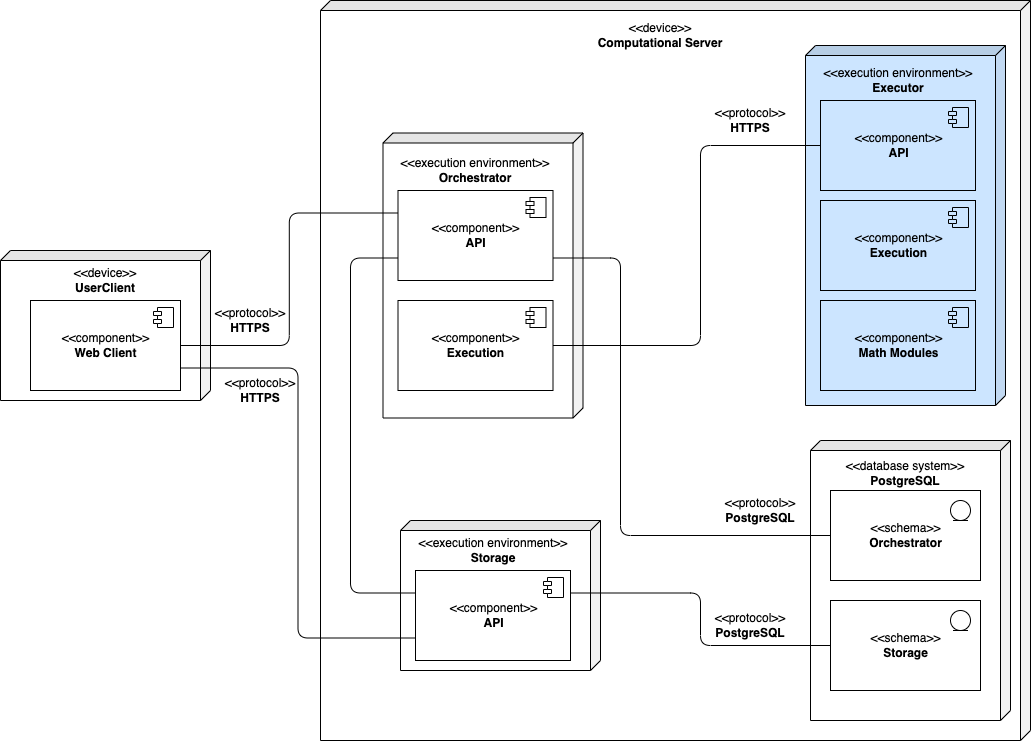
\includegraphics[width=\textwidth]{images/architecture/deployment_diagram}
	\caption{Диаграмма размещения}
	\label{pic:architecture__deployment-diagram}
\end{figure}
\vskip 5 mm

Расчетный сервис представлен тремя компонентами: API, расчётным модулем и математической библиотекой \textbf{nd\_plan}.
В качестве цели данной работы является проектирование и разработка API и расчетного модуля,
то поэтому только они и отражены на диаграммах ниже.

\begin{figure}[H]
	\hspace*{-2.5 cm}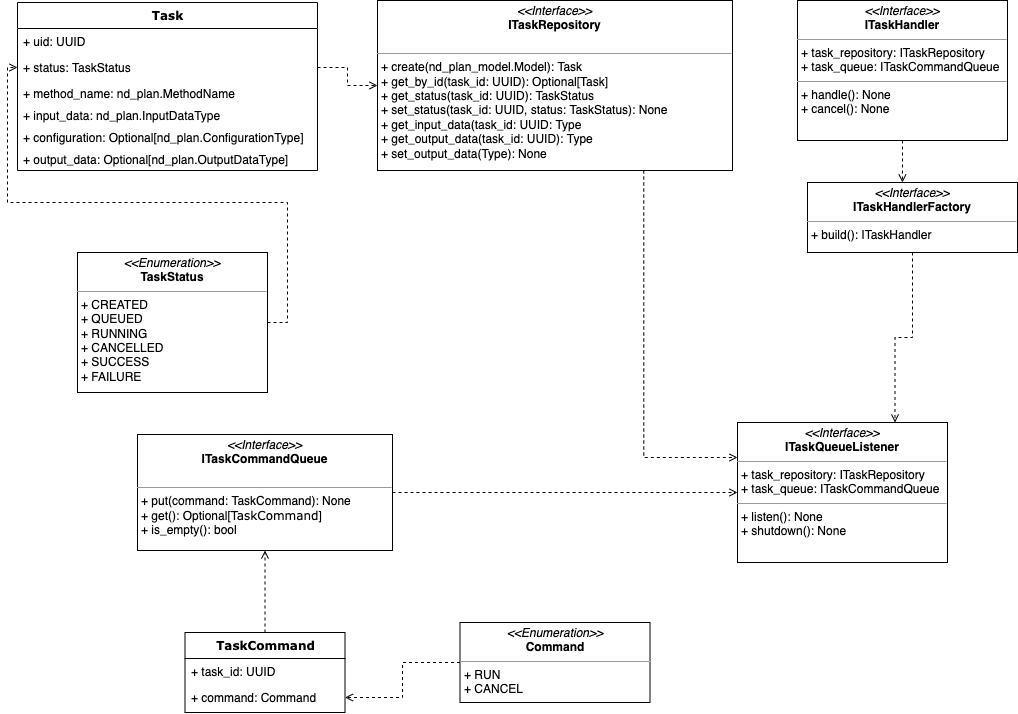
\includegraphics[width=1.2\textwidth]{images/architecture/execution_classes_diagram}
	\caption{Диаграмма классов расчетного модуля}
	\label{pic:architecture__execution-classes-diagram}
\end{figure}

\vskip 5 mm
Основное ядро бизнес-логики проекта представлено на диаграмме классов(см. рис\ \ref{pic:architecture__classes-diagram}).
Основные классы и интерфейсы:
\begin{enumerate}
	\item \textit{ITilesCacheStorage} -- сервис, отвечающий за кэширование векторных тайлов.
	\item \textit{ITilesRenderer} -- сервис, отвечающий за рендеринг векторных тайлов.
	\item \textit{ITilesDataProvider} -- сервис, отвечающий за получение данных из внешних источников для рендеринга.
	\item \textit{ITilesRepository} -- оркестратор, отвечает за получение отрендеренных тайлов.
	Если тайла нет в кэше, то он с помощью \textit{ITilesDataProvider} получает данные для рендеринга, потом
	с помощью \textit{ITilesRenderer} рендерит тайлы, а после сохраняет их в кэш \textit{ITilesCacheStorage}.
	\item \textbf{TileInfo} -- хранит в себе координаты запрашиваемого тайла, а также уникальный идентификатор генплана.
	\item \textbf{TileData} -- хранит в себе сырые данные, запрошенные по \textbf{TileInfo}.
	Из сырых данных генерируется \textbf{MapboxVectorTile}.
	\item \textbf{TileConfiguration} -- хранит в себе параметры слоев, которые требуется получить из источника данных.
	\item \textbf{MapboxVectorTile} -- хранит в себе данные, соответствующие спецификации \textit{Mapbox Vector Tile 2.1}.
\end{enumerate}


\begin{figure}[H]
	\hspace*{-2.5 cm}\includegraphics[width=1.2\textwidth]{images/architecture/}
	\caption{Диаграмма классов API}
	\label{pic:architecture__api-classes-diagram}
\end{figure}

\section*{\Large{РЕАЛИЗАЦИЯ}}
\addcontentsline{toc}{section}{РЕАЛИЗАЦИЯ}

При реализации описанной архитектуры была получена следующая структура
проекта(см. рисунок \ref{pic:implementation__packages}).

\begin{figure}[H]
	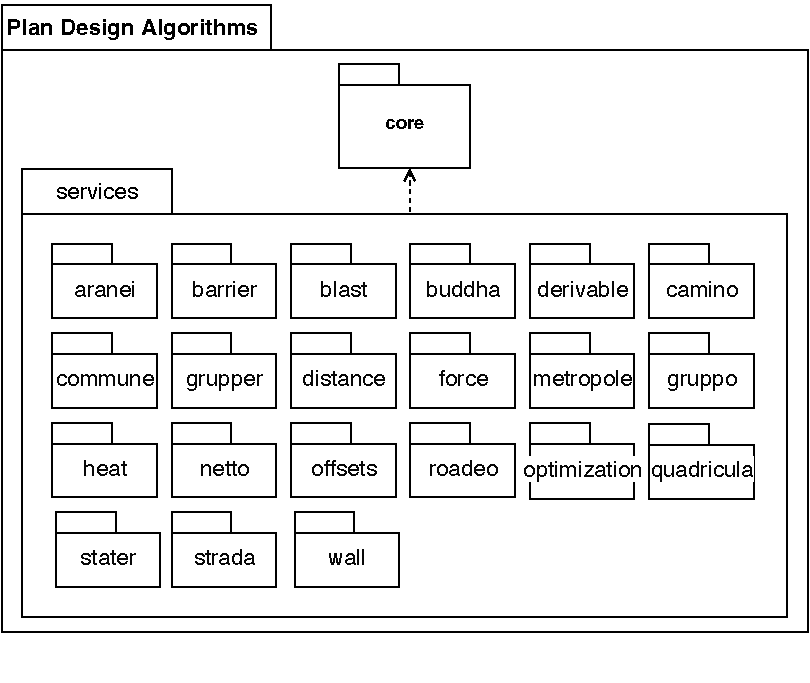
\includegraphics[width=0.6\textwidth]{pictures/packages}
	\caption{Диаграмма пакетов сервиса запуска расчётных задач}
	\label{pic:implementation__packages}
\end{figure}
\vskip 5 mm

Всего получилось 6 python-пакетов, в которых и скрыта основная логика работы.
\begin{enumerate}
    \item \textit{api} -- реализует API сервисы через HTTP. То есть endpoint-ы,
    модели запросов/ответов к серверу, а также взаимодействие с \textit{ITaskRepository} и \textit{ITaskDataManager}
    \item \textit{database} -- обеспечивает взаимодействие с базой данных.
    \item \textit{clients} -- пакеты, в котором находятся клиенты для взаимодействия с сервисами хранилища и сервиса 
    запуска математических методов.
    \item \textit{domain} -- пакет, в котором определены только интерфейсы взаимодействия между модулями программы.
    Непосредственная реализация обозначенных интерфейсов находится в других пакетах.
    \item \textit{execution} -- пакет, в котором находится код, отвечающий за запуск расчётных задач.
    \item \textit{repositories} -- пакет, который обеспечивает логику сохранения/получения сущностей проекта из БД.
\end{enumerate}

\subsection*{\Large{Примеры кода}}
\addcontentsline{toc}{subsection}{Примеры кода}

\begin{lstlisting}[language=Python, caption=main.py, captionpos=b]
from app import startup_app
import uvicorn

if __name__ == '__main__':
    app = startup_app()
    uvicorn.run(app, host="0.0.0.0", port=8080)
\end{lstlisting}

\vskip 10 mm
\begin{lstlisting}[caption=Dockerfile, captionpos=b]]
FROM python:3.8@sha256:4c4e6735f46e7727965d1523015874ab08f71377b3536b8789ee5742fc737059

WORKDIR /app

ENV LC_ALL C.UTF-8
ENV LANG C.UTF-8
ENV N_WORKERS 8

COPY requirements.txt .
RUN pip3 install --no-cache-dir -r requirements.txt

RUN pip3 check

COPY main.py .

COPY /app ./app

ENTRYPOINT /bin/bash -c "gunicorn run_app:app --workers=${N_WORKERS} --bind 0.0.0.0:8080 --worker-class aiohttp.GunicornWebWorker --timeout 0"
\end{lstlisting}

\vskip 10 mm
\begin{lstlisting}[language=Python, caption=domain/model.py, captionpos=b]
class Status(Enum):
    CREATED = "CREATED"
    QUEUED = "QUEUED"
    RUNNING = "RUNNING"
    CANCELLED = "CANCELLED"
    SUCCESS = "SUCCESS"
    FAILURE = "FAILURE"


@dataclass
class Feature:
    id: UUID = UUID(int=0)
    feature_type_id: UUID = UUID(int=0)


@dataclass
class Method:
    id: UUID = UUID(int=0)
    method_type_id: UUID = UUID(int=0)
    status: Status = Status.CREATED


@dataclass
class Calculation:
    id: UUID = UUID(int=0)
    calculation_type_id: UUID = UUID(int=0)
    status: Status = Status.CREATED


@dataclass
class Stage:
    id: UUID = UUID(int=0)
    stage_type_id: UUID = UUID(int=0)
    status: Status = Status.CREATED


@dataclass
class Task:
    id: UUID = UUID(int=0)
    name: str = ""
    task_type_id: UUID = UUID(int=0)
    status: Status = Status.CREATED
\end{lstlisting}
\vskip 10 mm

%\newpage
%\section*{\Large{Заключение}}
\addcontentsline{toc}{section}{Заключение}
В данной работе требовалось спроектировать и реализовать сервис, обеспечивающий
преобразование данных предметной области в объекты математической библиотеки \textbf{nd\_plan},
и имеющий возможность запускать методы данной библиотеки, учитывая особенности их выполнения.
С учетом функциональных и нефункциональных требований была спроектирована архитектура системы,
а так же эта архитектура была реализована.

%\newpage
%\addcontentsline{toc}{section}{Список использованных источников}
\begin{thebibliography}{8}
	\bibitem{CapitalBuilding} 
	«Градостроительный кодекс Российской Федерации» от 29.12.2004 N 190-ФЗ (ред. от 31.12.2017)
	\bibitem{SafetyBuildings}
	Федеральный закон «Технический регламент о безопасности зданий и сооружений» от 30.12.2009 N 384-ФЗ.
	\bibitem{CivilCode}
	«Гражданский кодекс Российской Федерации (часть первая)» от 30.11.1994 N 51-ФЗ (ред. от 06.04.2011), Статья 233
	\bibitem{Fire}
	«CВОД ПРАВИЛ СП 4.13130.2013
	СИСТЕМЫ ПРОТИВОПОЖАРНОЙ ЗАЩИТЫ
	ОГРАНИЧЕНИЕ РАСПРОСТРАНЕНИЯ ПОЖАРА НА ОБЪЕКТАХ ЗАЩИТЫ
	ТРЕБОВАНИЯ
	К ОБЪЕМНО-ПЛАНИРОВОЧНЫМ И КОНСТРУКТИВНЫМ РЕШЕНИЯМ» от 24.06.2013
	\bibitem{PythonReference} Python 3.8 Documentation [Интернет ресурс]:\\
	\url{URL:https://docs.python.org/3.8/}(дата обращения: 28.01.22)
	\bibitem{PythonProsAndCons} Python Advantages and Disadvantages [Интернет ресурс]:\\
	\url{URL:https://techvidvan.com/tutorials/python-advantages-and-disadvantages/} (дата обращения: 28.01.22)
	\bibitem{PostGIS} PostGIS Reference [Интернет ресурс]:\\
	\url{URL:https://postgis.net/documentation/} (дата обращения: 28.01.22)
	\bibitem{ArtOfTesting}
	Glenford J. Myers, Corey Sandler, Tom Badgett "The Art of Software Testing", 3rd Edition, 16 Dec 2011
	\bibitem{Docker} Docker Reference[Интернет ресурс]:\\
	\url{URL:https://docs.docker.com} (дата обращения: 28.01.22)
	\bibitem{Sphinx} Sphinx Python Documentation [Интернет ресурс]:\\
	\url{URL:https://www.sphinx-doc.org/en/master/} (дата обращения: 28.01.22)
	\bibitem{Protobuf} Protobuf Documentation [Интернет ресурс]:\\
	\url{https://developers.google.com/protocol-buffers/docs/overview} (дата обращения: 28.01.22)
	\bibitem{DesignPatterns}
	Erich Gamma, Richard Helm, Ralph Johnson, John Vlissides
	"Design Patterns: Elements of Reusable Object-Oriented Software", 1st Edition
	\bibitem{CleanCode}
	Martin Robert C. "Clean Code: A Handbook of Agile Software Craftsmanship" Aug 1, 2008
\end{thebibliography}

\end{document}
